\chapter{Approach}
\label{ch:approach}
%%%%%%%%%%%%%%%%%%%%%%%
% - description of the designed system
% - analysis and review of the current software architecture
% - gerne in die Tiefe gehen
%%%%%%%%%%%%%%%%%%%%%%%

In this chapter we give an overview of the current software architecture on which the Basilisk platform is build.
\\

The main idea for the Basilisk platform is that a user can register a \ts{} for a continuous benchmark by setting up a hook to the repository on GitHub or a docker image from Docker Hub containing the \ts{}, which will then be observed by Basilisk.
If there is a new release of the \ts{}, Basilisk will fetch and build the new docker container to perform a benchmark.
The measured results of the benchmark will be stored in a database and are then available through the web frontend to review.
\todo[inline]{right position for this explanation?}


The basic architecture pattern of the Basilisk platform is the microservice architecture (see chapter \ref{sec:microservice_architecture} for a short description). 
This means that the platform is divided into multiple services on which the workload and the different tasks are divided.
The services can be run on different hardware systems and they interact with each other via a message queue system.
\\

Figure \ref{fig:basilisk_high_level_design} gives an overview of the microservice architecture for the Basilisk platform and the most important messages send between the services.
\todo{graphic}
\begin{figure}[tbph]
	\centering
	\textbf{TODO: better graphic}
	%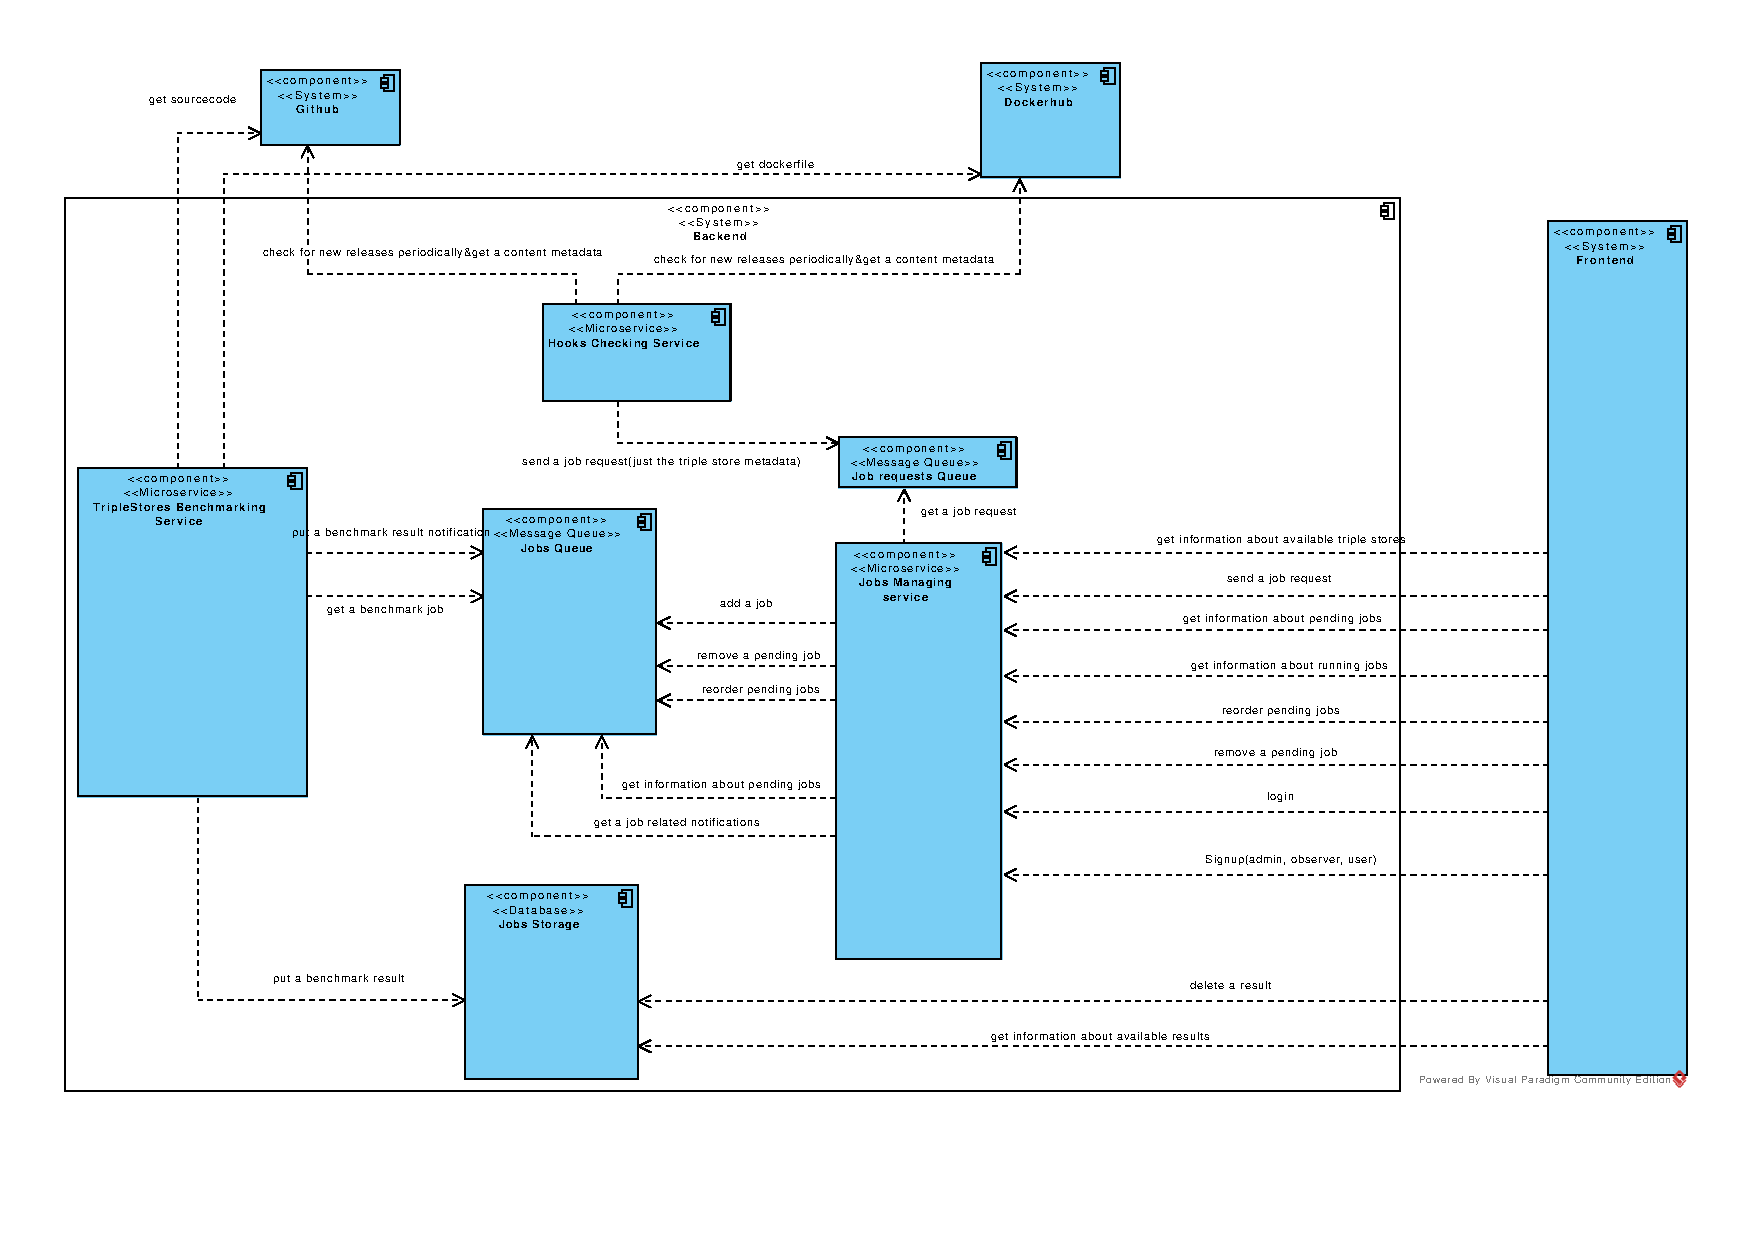
\includegraphics[width=1.1\textwidth]{figures/basilisk_high_level_design.pdf}
	\caption{High level design of the Basilisk framework}
	\label{fig:basilisk_high_level_design}
\end{figure}
\\

\section{Main Services}
\label{sec:main_services}
The next sections explain the three main services, namely \acl{hcs} (\ref{sec:hooks_checking_service}), \acl{jms} (\ref{sec:jobs_managing_service}), and \acl{tbs} (\ref{sec:ts_benchmarking_service}).

This explanation follows the flow of actions that happen while configuring a continuous benchmark and the actions that happen when a benchmark is initiated.


\subsection{\acl{hcs}}
\label{sec:hooks_checking_service}
The main task of the \ac{hcs} is to observe Github and Docker Hub repositories for new releases or changes.

When a user wants to set up a new continuous benchmark, the \ac{hcs} needs to be informed which repository (GitHub or Docker Hub) needs to be observed for changes.
This happens through API calls from the frontend to the hooks checking service providing the repository name and owner.
The \ac{hcs} will then create a hook for the repository to get notice about changes.
A hook is in general a piece of code or software that attaches itself to a software component to intercept messages and react to those messages, \eg, with function calls.
In the case of the \ac{hcs} the hooks can be seen as bookmarks for the repositories to regularly check for new versions and releases.
Each hook stores the latest known version of an repository to easily compare for new versions.

When the \ac{hcs} notices a new release for a repository it observes, it updates the corresponding hook to the newest version and sends a message about the new version to the \acl{jrq} from which the \acl{jms} retrieves the message.

\subsubsection{API}
\label{sec:hooks_api}


\subsection{\acl{jms}}
\label{sec:jobs_managing_service}
The \acf{jms} processes the requests coming from the web-frontend, checks if the Hooks Checking Service has found a new version for a benchmark and creates jobs for new benchmarks.

\subsubsection{API}
\label{sec:jobs_api}


\subsection{\acl{tbs}}
\label{sec:ts_benchmarking_service}
Lastly the \ac{tbs} executes the benchmarks given to it and saves the results to a database.

\subsubsection{API}
\label{sec:benchmarking_api}


\section{Message Queue System}
\label{sec:message_queue}
The messages send between the services are transmitted via the RabbitMQ\footnote{\url{https://www.rabbitmq.com/}} message broker software.


\section{Programming Language and Frameworks}
\label{sec:prog_lang_and_framework}
All services are implemented with Java and are using the Spring Boot framework.

\subsection{Package Structure}
\label{sec:folder_structure}
The package structure used for the service implementation is similar in all three services.
It is strongly influence through the use of the Spring Boot framework.
The Spring and Spring Boot framework are shortly described in chapter \ref{sec:spring}.
In the following the most important packages of the services are described.

\paragraph{config}
In the config folder important Spring Beans are defined and configured.
Also the configuration for the RabbitMQ message queues is defined here.
The classes in this package are marked with the @Configuration annotation which informs the Spring framework that these classes declare @Bean methods for generating Spring Beans.
Beans are defined in Spring as the objects that form the backbone of the application.

\paragraph{core}



\section{Frontend}
\label{sec:frontend}